%% \documentclass[handout,t]{beamer} % HANDOUT
%% \documentclass[handout,notes=show,t]{beamer} % NOTES
\documentclass[t]{beamer} % SLIDES

\usetheme{SIGIL}
\usepackage{beamer-tools-sigil}

%%
%% some useful macros: mathematical notation etc.
%%

%% abbreviations for logic symbols
\renewcommand{\implies}{\Rightarrow}
\newcommand{\equivalent}{\Leftrightarrow}

%% abbreviations for common number spaces
\newcommand{\setN}[1][]{\mathbb{N}_{#1}} % allows \setN and \setN[0]
\newcommand{\setZ}{\mathbb{Z}}
\newcommand{\setQ}{\mathbb{Q}}
\newcommand{\setR}{\mathbb{R}}

%% sets and (sub-)sets defined by condition
\newcommand{\set}[1]{\{#1\}}
\newcommand{\setdef}[2]{\set{#1\,|\,#2}}
\newcommand{\bigset}[1]{\bigl\{#1\bigr\}}
\newcommand{\bigsetdef}[2]{\bigset{#1\bigm|#2}}
\newcommand{\setscale}[1]{\left\{#1\right\}}
\newcommand{\setdefscale}[2]{\setscale{#1\left|\,#2\right.}}

%% absolute value and norm
\newcommand{\abs}[1]{\lvert #1\rvert}
\newcommand{\bigabs}[1]{\bigl\lvert #1\bigr\rvert}
\newcommand{\absscale}[1]{\left\lvert #1\right\rvert}
\newcommand{\norm}[2][]{\lVert #2\rVert_{#1}}
\newcommand{\bignorm}[2][]{\bigl\lVert #2\bigr\rVert_{#1}}
\newcommand{\normscale}[2][]{\left\lVert #2\right\rVert_{#1}}

%% complement set (with optional index)
\newcommand{\compl}[1][]{\mathcal{C}^{#1}}

%% power set: \powerset{\Sigma^*}
\newcommand{\powerset}[1]{\mathcal{P}(#1)}

%% uparrow: a \ua b = direct dominance in ordered tree
\newcommand{\ua}{\uparrow}

%% left-right arrow: this $\lra$ that
\newcommand{\lra}{\leftrightarrow}

%% expanded engineering notation: 4.2\x\e+5
\newcommand{\e}[2]{10^{\ifthenelse{\equal{#1}{+}}{}{#1}#2}}
\newcommand{\x}{\cdot}

%% arg max & min: \argmax_{x\in C}, \argmin_{x\in C}
\newcommand{\argmax}{\mathop{\text{arg~max}}}
\newcommand{\argmin}{\mathop{\text{arg~min}}}

%% infinitesimal elements: \dx, \dy = \dX{y}, \dz
\newcommand{\dX}[1]{\,\mathit{d{#1}}}
\newcommand{\dx}{\dX{x}}
\newcommand{\dy}{\dX{y}}
\newcommand{\dz}{\dX{z}}

%%% Local Variables: 
%%% mode: latex
%%% TeX-master: ""
%%% End: 
  % basic mathematical notation
%%
%% some useful macros: statistical notation
%%

%% \p{X=k};  \pC{X=k}{Y=l};  \bigp{X_i = k};   \pscale{\frac{Z}{S^2}};
%% probability P(X=k) and conditional probability P(X=k|Y=l), also with larger or scaled parentheses
%% \p[\theta]{X=k};  \pC[\text{interpolated}]{X=k}{Y=l};  ...
%% with optional subscripts (for model probability, null probability, etc.)
\newcommand{\p}[2][]{\mathop{\mathrm{Pr}_{#1}}(#2)}
\newcommand{\pscale}[2][]{\mathop{\mathrm{Pr}_{#1}}\!\left(#2\right)}
\newcommand{\bigp}[2][]{\mathop{\mathrm{Pr}_{#1}}\bigl(#2\bigr)}
\newcommand{\pC}[3][]{\p[#1]{#2\,|\,#3}} 
\newcommand{\pCscale}[3][]{\pscale[#1]{#2\left|\,#3\right.\!}} 
\newcommand{\bigpC}[3][]{\bigp[#1]{#2\!\bigm|\!#3}} 

%% \Exp{X};  \Var{X};  \Exp[0]{X};  \Var[0]{X};  
%% \bigExp{X}; \bigVar{X}; \Expscale{X};  \Varscale{X};
%% expectation E[X] and variance V[X], expectation and variance under null hypothesis, 
%% and variants with largeer or scaled brackets
\newcommand{\Exp}[2][]{\mathrm{E}_{#1}[#2]}
\newcommand{\Var}[2][]{\mathop{\mathrm{Var}}_{#1}[#2]}
\newcommand{\bigExp}[2][]{\mathrm{E}_{#1}\!\bigl[#2\bigr]}
\newcommand{\bigVar}[2][]{\mathop{\mathrm{Var}}_{#1}\bigl[#2\bigr]}
\newcommand{\Expscale}[2][]{\mathrm{E}_{#1}\left[#2\right]}
\newcommand{\Varscale}[2][]{\mathop{\mathrm{Var}}_{#1}\left[#2\right]}

%% \pihat = \hat{\pi}
%% sampling estimate for population probability \pi (may need fine-tuning)
\newcommand{\pihat}{\hat{\pi}}

%% \Entropy{X}, \Entropy{p}, \KL{p}{q}, \MI{X}{Y}
%% \bigEntropy{}, \Entropyscale{}, \bigKL{}{}, \KLscale{}{}, \bigMI{}{}, \MIscale{}{}
%% entropy, KL distance, conditional entropy and mutual information (with scaled variants)
\newcommand{\Entropy}[1]{H[{#1}]}
\newcommand{\bigEntropy}[1]{H\bigl[{#1}\bigr]}
\newcommand{\Entropyscale}[1]{H\left[{#1}\right]}
\newcommand{\KL}[2]{D({#1}\|{#2})}
\newcommand{\bigKL}[2]{D\bigl({#1}\bigm\|{#2}\bigr)}
\newcommand{\KLscale}[2]{D\left({#1}\left\|{#2}\right.\right)}
\newcommand{\MI}[2]{I[{#1};{#2}]}
\newcommand{\bigMI}[2]{I\bigl[{#1};{#2}\bigr]}
\newcommand{\MIscale}[2]{I\left[{#1};{#2}\right]}

%% \corr (correlation) and \cov (covariance) as mathop's
\newcommand{\corr}{\mathop{\mathrm{corr}}}
\newcommand{\cov}{\mathop{\mathrm{cov}}
}
%%% Local Variables: 
%%% mode: latex
%%% TeX-master: ""
%%% End: 
  % notation for probability theory and statistics
%%
%% convenience macros for linear algebra (vectors and matrices)
%%

%% \Vector[i]{x} ... vector variable with optional _superscript_ index in parentheses
%% \Vector[']{x} ... special case: ' superscript not enclosed in parentheses
%% \vx, \vy, \vz ... abbreviations for common vector names
\newcommand{\Vector}[2][]{\mathbf{#2}\ifthenelse{\equal{#1}{}}{}{^{(#1)}}}
\newcommand{\vx}[1][]{\Vector[#1]{x}}
\newcommand{\vy}[1][]{\Vector[#1]{y}}
\newcommand{\vz}[1][]{\Vector[#1]{z}}
\newcommand{\vu}[1][]{\Vector[#1]{u}}
\newcommand{\vv}[1][]{\Vector[#1]{v}}
\newcommand{\vw}[1][]{\Vector[#1]{w}}
\newcommand{\vm}[1][]{\Vector[#1]{m}} 
\newcommand{\va}[1][]{\Vector[#1]{a}} % vectors of coefficients
\newcommand{\vb}[1][]{\Vector[#1]{b}} % for basis
\newcommand{\ve}[1][]{\Vector[#1]{e}} % for standard basis of R^n
\newcommand{\vn}[1][]{\Vector[#1]{n}} % normal vector
\newcommand{\vnull}[1][]{\Vector[#1]{0}} % neutral element

%% \Span{\vb[1],\ldots,\vb[k]} ... span of set of vectors
%% \Rank{...} ... rank of set of vectors or matrix
%% \Det{...}, \det A ... determinant of a set of vectors / a matrix A
%% \Image{f}, \Kernel{f} ... image and kernel of a linear map
\newcommand{\Span}[1]{\mathop{\text{sp}}\left(#1\right)}
\newcommand{\Rank}[1]{\mathop{\text{rank}}\left(#1\right)}
\newcommand{\Det}[1]{\mathop{\text{Det}}\left(#1\right)}
%% \det is already defined in the standard library
\newcommand{\Image}[1]{\mathop{\text{Im}}\left(#1\right)}
\newcommand{\Kernel}[1]{\mathop{\text{Ker}}\left(#1\right)}

%% \dist[2]{\vx}{\vy} ... distance between two vectors (p-metric)
\newcommand{\dist}[3][]{d_{#1}\left(#2, #3\right)}
\newcommand{\bigdist}[3][]{d_{#1}\bigl(#2, #3\bigr)}

%% \sprod{\vu}{\vv} ... scalar product
\newcommand{\sprod}[2]{\left\langle #1, #2 \right\rangle}
\newcommand{\bigsprod}[2]{\bigl\langle #1, #2 \bigr\rangle}


%%% Local Variables: 
%%% mode: latex
%%% TeX-master: ""
%%% End: 
% convenience macros for vectors and matrices

%%%
%%% local configuration adjustments
%%%

%%% You can change pre-defined colours here, override built-in macros from the
%%% style definition and standard library, as well as define macros needed by
%%% all local documents.

%%% e.g. adjust counterpoint (dark green) for data projectors where greens are
%%% far too bright, as well as green component of light colour and pure green
%%% (of course, it's a better solution to adjust the gamma settings of your monitor)
%%
%% \definecolor{counterpoint}{rgb}{.1, .3, 0}
%% \definecolor{light}{rgb}{.45, .3, .55}
%% \definecolor{puregreen}{rgb}{0, .35, 0}

%% ----- extra packages we need to load

\usepackage{tikz}
\usepackage{alltt}              % code examples with nicely formatted comments
\usepackage{rotating}


%% ----- author and copyright messages (so updates are automatically inserted into all files)
\newcommand{\sigilauthors}{%
  \author[SIGIL]{Designed by Stefan Evert\inst{1} and Marco Baroni\inst{2}}
  \institute[Evert \& Baroni]{
    \inst{1}Computational Corpus Linguistics Group\\
    Friedrich-Alexander-Universit�t Erlangen-N�rnberg, Germany
    \and
    \inst{2}Center for Mind/Brain Sciences (CIMeC)\\
    University of Trento, Italy
  }
}
\newcommand{\sigilcopyright}{%
  \date[sigil.r-forge.r-project.org]{%
    \primary{\footnotesize\url{http://SIGIL.r-forge.r-project.org/}}\\
    \light{\tiny Copyright \textcopyright\ 2007--2018 Evert \& Baroni}}
}

%% ----- automatically show TOC reminder at beginning of each subsection
\AtBeginSubsection[]
{
  \begin{frame}
    \frametitle{Outline}
    \tableofcontents[current,currentsubsection]
  \end{frame}
}

%% ----- some useful macros for the SIGIL course

\newenvironment{Rcode}[1][]{%
  \setbeamercolor{block title}{fg=counterpoint,bg=counterpoint!15!white}%
  \setbeamercolor{block body}{bg=counterpoint!5!white}\small%
  \begin{block}{#1}\begin{alltt}\ungap[1]}{%
      \ungap[1]\end{alltt}\end{block}} % \end{alltt} ... to deconfuse emacs

%% use \sbox{\Rbox} ... \usebox{\Rbox} to insert arbitray latex into Rcode environment
\newsavebox{\Rbox}

%% > plot(x,y)      \REM{this produces a scatterplot}
\newcommand{\REM}[2][\small]{\textsf{#1\color{primary}\# #2}}

%% nice colour for R output: \begin{Rout} .. \end{Rout}
\newenvironment{Rout}[1][\footnotesize]{%
  \begin{footnotesize}#1\color{secondary}\bfseries}{%
    \color{black}\mdseries\end{footnotesize}}

%% rotated column labels for table (to fit long text into narrow columns
\newcommand{\rotLabel}[2][60]{\begin{rotate}{#1}#2\end{rotate}}
 % local adjustments to configuration and macros

%%%%%%%%%%%%%%%%%%%%%%%%%%%%%%%%%%%%%%%%%%%%%%%%%%%%%%%%%%%%%%%%%%%%%%
%% Titlepage

\title[3b.\ Continuous Data: Inference]{Unit 3: Inferential Statistics for Continuous Data}
\subtitle{Statistics for Linguists with R -- A SIGIL Course}
\sigilauthors
\date[sigil.r-forge.r-project.org]{%
  \light{\tiny \sigilcopyright}}

\begin{document}

\frame{\titlepage}

%%%%%%%%%%%%%%%%%%%%%%%%%%%%%%%%%%%%%%%%%%%%%%%%%%%%%%%%%%%%%%%%%%%%%%

\section*{Outline}
\frame{ 
  \frametitle{Outline}
  \tableofcontents
}

%%%%%%%%%%%%%%%%%%%%%%%%%%%%%%%%%%%%%%%%%%%%%%%%%%%%%%%%%%%%%%%%%%%%%%
\section{Inferential statistics}

%%%%%%%%%%%%%%%%%%%%%%%%%%%%%%%%%%%%%%%%%%
\subsection{Preliminaries}

\begin{frame}
  \frametitle{Inferential statistics for continuous data}
  % \framesubtitle{}

  \begin{itemize}
  \item Goal: infer (characteristics of) population distribution from small
    random sample, or test hypotheses about population
    \begin{itemize}
    \item problem: overwhelmingly infinite coice of possible distributions
    \item can estimate/test characteristics such as mean $\mu$ and s.d.\ $\sigma$
    \item but $H_0$ doesn't determine a unique sampling distribution then
    \item[\hand] \h{parametric} model, where the population distribution of a
      r.v.\ $X$ is completely determined by a small set of parameters
    \item[]
    \end{itemize}
  \item<2-> In this session, we assume a \h{Gaussian population} distribution%
    \begin{itemize}
    \item estimate/test parameters $\mu$ and $\sigma$ of this distribution 
    \item sometimes a scale transformation is necessary (e.g.\ lognormal)
    \item[]
    \end{itemize}
  \item<3-> Nonparametric tests need fewer assumptions, but \ldots
    \begin{itemize}
    \item cannot test hypotheses about $\mu$ and $\sigma$\\
      (instead: median $m$, IQR = inter-quartile range, etc.)
    \item more complicated and computationally expensive procedures
    \item correct interpretation of results often difficult
    \end{itemize}
  \end{itemize}
\end{frame}

\begin{frame}
  \frametitle{Inferential statistics for continuous data}
  % \framesubtitle{}

  Rationale similar to binomial test for frequency data:
  measure observed \h{statistic} $T$ in sample, which is compared against its
  \h{expected} value $\Exp[0]{T}$ \so if difference is large enough, reject $H_0$
  \begin{itemize}
  \item[]
  \item<2-> Question 1: What is a suitable statistic?
    \begin{itemize}
    \item depends on null hypothesis $H_0$
    \item large difference $T - \Exp[0]{T}$ should provide evidence against $H_0$
    \item e.g.\ unbiased estimator for population parameter to be tested
    \end{itemize}
  \item[]
  \item<3-> Question 2: what is ``large enough''?
    \begin{itemize}
    \item reject if difference is unlikely to arise by chance
    \item need to compute sampling distribution of $T$ under $H_0$
    \end{itemize}
  \end{itemize}
\end{frame}

\begin{frame}
  \frametitle{Inferential statistics for continuous data}
  % \framesubtitle{}
  
  \begin{itemize}
  \item Easy if statistic $T$ has a Gaussian distribution $T \sim N(\mu, \sigma^2)$
    \begin{itemize}
    \item $\mu$ and $\sigma^2$ are determined by null hypothesis $H_0$
    \item reject $H_0$ at two-sided significance level $\alpha = .05$\\
      if $T < \mu - 1.96\sigma$ or $T > \mu + 1.96\sigma$
    \end{itemize}
  \end{itemize}

  \begin{columns}[b]
    \begin{column}{55mm}
      \begin{itemize}
      \item<2-> This suggests a standardized \h{z-score} as a measure of extremeness:
        \[
        Z \coloneq \frac{T - \mu}{\sigma}
        \]
      \item<2-> Central range of sampling variation: $\abs{Z} \leq 1.96$
      \end{itemize}
    \end{column}
    \begin{column}{45mm}
    \hspace*{-1cm}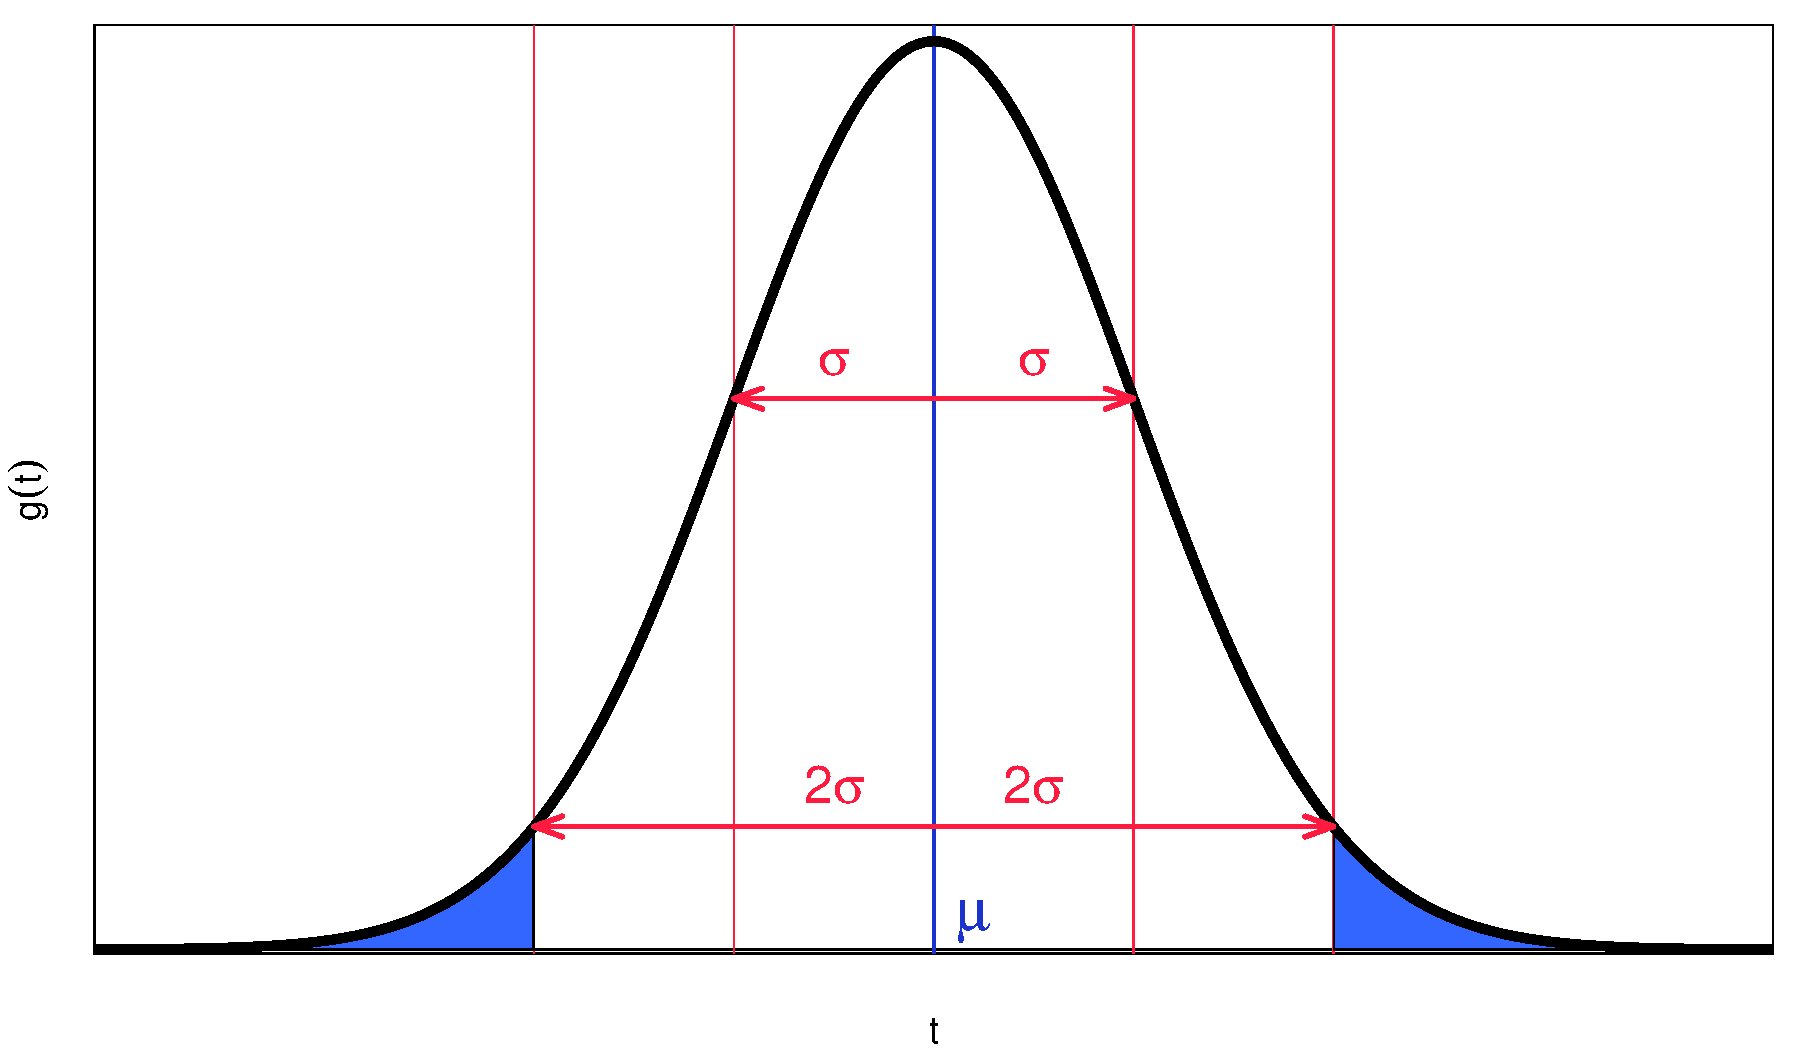
\includegraphics[width=55mm]{img/gaussian_parameters}      
    \end{column}
  \end{columns}
\end{frame}

\begin{frame}
  \frametitle{Notation for random samples}
  % \framesubtitle{}

  \begin{itemize}
  \item Random sample of $n \ll m = \abs{\Omega}$ items
    \begin{itemize}
    \item e.g.\ participants of survey, Wikipedia sample, \ldots
    \item recall importance of completely random selection
    \end{itemize}
  \item Sample described by observed values of r.v.\ $X, Y, Z, \ldots$:
    \[
    x_1, \ldots, x_n; \quad y_1, \ldots, y_n; \quad z_1, \ldots, z_n
    \]
    \ungap[1]
    \begin{itemize}
    \item[\hand] specific items $\omega_1, \ldots, \omega_n$ are irrelevant,
      we are only interested in their properties $x_i = X(\omega_i)$,
      $y_i = Y(\omega_i)$, etc.
    \end{itemize}
    \pause
  \item Mathematically, $x_i, y_i, z_i$ are realisations of random variables
    \[
    X_1, \ldots, X_n; \quad Y_1, \ldots, Y_n; \quad Z_1, \ldots, Z_n
    \]
  \item $X_1,\ldots, X_n$ are independent from each other and each one has the
    same distribution $X_i \sim X$ \so \h{i.i.d.} random variables
    \begin{itemize}
    \item[\hand] each random experiment now yields complete sample of size $n$
    \end{itemize}
  \end{itemize}

\end{frame}

%%%%%%%%%%%%%%%%%%%%%%%%%%%%%%%%%%%%%%%%%%%%%%%%%%%%%%%%%%%%%%%%%%%%%%
\section{One-sample tests}

%%%%%%%%%%%%%%%%%%%%%%%%%%%%%%%%%%%%%%%%%%
\subsection{Testing the mean}

\begin{frame}
  \frametitle{A simple test for the mean}
  % \framesubtitle{}

  \begin{itemize}
  \item Consider simplest possible $H_0$: a \h{point hypothesis}
    \[
    H_0:\;\; \mu = \mu_0,\; \sigma = \sigma_0
    \]
    \ungap[1]
    \begin{itemize}
    \item[\hand] together with normality assumption, population distribution
      is completely determined
    \end{itemize}
  \item How would you test whether $\mu = \mu_0$ is correct?%
    \pause
  \item An intuitive test statistic is the \h{sample mean}
    \[
    \bar{x} = \frac{1}{n} \sum_{i=1}^n x_i
    \qquad \text{with} \qquad
    \bar{x}\approx \mu_0 \text{ under } H_0
    \]
  \item Reject $H_0$ if difference $\bar{x} - \mu_0$ is sufficiently large
    \begin{itemize}
    \item[\hand] need to work out sampling distribution of $\bar{X}$
    \end{itemize}
  \end{itemize}

\end{frame}

\begin{frame}
  \frametitle{The sampling distribution of $\bar{X}$}
  % \framesubtitle{}

  \begin{itemize}
  \item The sample mean is also a random variable:
    \[
    \bar{X} = \frac{1}{n} \bigl( X_1 + \dots + X_n \bigr)
    \]
  \item $\bar{X}$ is a sensible test statistic for $\mu$ because it is \h{unbiased}:
    \[
    \Exp{\bar{X}} = \Expscale{ \frac{1}{n} \sum_{i=1}^n X_i }
    = \frac{1}{n} \sum_{i=1}^n \Exp{X_i} 
    = \frac{1}{n} \sum_{i=1}^n \mu = \mu
    \]
    \pause
  \item An important property of the Gaussian distribution: if $X \sim N(\mu_1,
    \sigma^2_1)$ and $Y \sim N(\mu_2, \sigma^2_2)$ are \primary{independent}, then
    \begin{align*}
      X + Y &\sim N(\mu_1 + \mu_2, \sigma^2_1 + \sigma^2_2)\\
      r\cdot X &\sim N(r\mu_1, r^2 \sigma^2_1) \quad \text{ for } r\in \setR
    \end{align*}
  \end{itemize}
  \addnote{The first question is whether it makes sense to base our test for
    the mean on the sample average, i.e.\ whether $\bar{X}$ is a sensible test
    statistic for $\mu$.}%
  \addnote{To answer this question, we need to work out (properties of) the
    sampling distribution of $\bar{X}$ across different random samples of the
    same size $n$.}%
  \addnote{A minimal requirement is \emph{unbiasedness}: the test statistic
    should not systematically indicate a wrong value for $\mu$ (possibly after
    suitable rescaling: $\bar{X} - \mu$ would be just as sensible as a test
    statistic).}%
  \addnote{Unbiasedness is not sufficient to ensure that a test based on
    $\bar{X}$ is reliable.  We also need to know the variability of $\bar{X}$,
    or preferably its complete sampling distribution.}%
  \addnote{An important advantage of Gaussian random variables is that
    $\bar{X}$ also follows a Gaussian distribution.  There are only very few
    other distributions with this property (e.g.\ Cauchy).}%
\end{frame}

\begin{frame}
  \frametitle{The sampling distribution of $\bar{X}$}
  % \framesubtitle{}

  \begin{itemize}
  \item Since $X_1, \ldots, X_n$ are i.i.d.\ with $X_i\sim N(\mu, \sigma^2)$,
    we have
    \begin{gather*}
      X_1 + \dots + X_n \sim N(n \mu, n \sigma^2) \\
      \bar{X} = \frac{1}{n} \bigl( X_1 + \dots + X_n \bigr) 
      \sim N(\mu, \frac{\sigma^2}{n})
    \end{gather*}
  \item $\bar{X}$ has Gaussian distribution with same mean $\mu$ but smaller s.d.\
    than the original r.v.\ $X$: $\sigma_{\bar{X}} = \sigma / \sqrt{n}$
    \begin{itemize}
    \item[\hand] explains why normality assumptions are so convenient
    \item[\hand] larger samples allow more reliable hypothesis tests about $\mu$
    \item[]
    \end{itemize}
    \pause
  \item If the sample size $n$ is large enough, $\sigma_{\bar{X}} = \sigma /
    \sqrt{n} \to 0$\\ and the sample mean $\bar{x}$ becomes an accurate estimate
    of the true population value $\mu$ (\h{law of large numbers})
  \end{itemize}
\end{frame}

\begin{frame}
  \frametitle{The $z$ test}
  % \framesubtitle{}

  \begin{itemize}
  \item Now we can quantify the extremeness of the observed value $\bar{x}$,
    given the null hypothesis $H_0: \mu=\mu_0, \sigma=\sigma_0$
    \[
    z = \frac{\bar{x} - \mu_0}{\sigma_{\bar{X}}}
     = \frac{\bar{x} - \mu_0}{\sigma_0 / \sqrt{n}}
    \]
  \item Corresponding r.v.\ $Z$ has a standard normal distribution if $H_0$ is
    correct: $Z \sim N(0,1)$%
    \pause
  \item We can reject $H_0$ at significance level $\alpha$ if
    \[
    \begin{array}{c ccc @{\hspace{1cm}} c}
      \alpha = & .05 & .01 & .001 & \\
      \abs{z} > & 1.960 & 2.576 & 3.291 & \text{\secondary{\texttt{-qnorm($\alpha$/2)}}}
    \end{array}
    \]
    \pause\ungap
  \item Two problems of this approach:
    \begin{enumerate}
    \item need to make hypothesis about $\sigma$ in order to test $\mu=\mu_0$
    \item $H_0$ might be rejected because of $\sigma \gg \sigma_0$ even if
      $\mu=\mu_0$ is true
    \end{enumerate}
  \end{itemize}
  \addnote{Recall that sampling distribution of $\bar{X}$ describes how the
    sample average varies across different random samples of the same size $n$
    from the same population satisfying $H_0$ (think of many sociologists
    taking surveys of 100 random people each).}%
  \addnote{We reject $H_0$ if the observed value of $\bar{X}$ is sufficiently
    improbable according to the sampling distribution, i.e.\ unlikely to
    happen by chance if $H_0$ were true.}%
  \addnote{Note that for the binomial test in Unit~2, the sampling
    distribution of the passive count $X$ was discrete.  Now the test
    statistic $\bar{X}$ has a continuous distribution described by a density
    function.}%
  \addnote{R function \texttt{qnorm} and other functions for working with
    probability distributions will be explained in a moment.}%
  \addnote{If we overestimate $\sigma\ll \sigma_0$, the $z$ test might fail to
    reject $\mu=\mu_0$ even though it clearly isn't true.}%
\end{frame}

%%%%%%%%%%%%%%%%%%%%%%%%%%%%%%%%%%%%%%%%%%
\subsection{Testing the variance}

\begin{frame}
  \frametitle{A test for the variance}
  % \framesubtitle{}

  \begin{itemize}
  \item An intuitive test statistic for $\sigma^2$ is the error sum of squares
    \[
    V = (X_1 - \mu)^2 + \dots + (X_n - \mu)^2
    \]
  \item Squared error $(X - \mu)^2$ is $\sigma^2$ on average \so
    $\Exp{V} = n \sigma^2$
    \begin{itemize}
    \item reject $\sigma = \sigma_0$ if $V\gg n \sigma^2_0$ (variance larger than expected)
    \item reject $\sigma = \sigma_0$ if $V\ll n \sigma^2_0$ (variance smaller than expected)
    \item[\hand] sampling distribution of $V$ shows if difference is large
      enough
    \end{itemize}
    \pause
  \item Rewrite $V$ in the following way:
    \begin{align*}
      V &= \sigma^2 \left[
        \left( \frac{X_1 - \mu}{\sigma} \right)^2 + \dots 
        + \left( \frac{X_n - \mu}{\sigma} \right)^2
      \right] \\
      &= \sigma^2 (Z_1^2 + \dots + Z_n^2)
    \end{align*}
    with $Z_i\sim N(0,1)$ i.i.d.\ standard normal variables
  \end{itemize}
\end{frame}

\begin{frame}
  \frametitle{A test for the variance}
  % \framesubtitle{}
  
  \begin{itemize}
  \item Note that the distribution of $Z_1^2 + \dots + Z_n^2$ does not depend
    on the population parameters $\mu$ and $\sigma^2$ (unlike $V$)
  \item Statisticians have worked out the distribution of $\sum_{i=1}^n Z_i^2$
    for i.i.d.\ $Z_i\sim N(0,1)$, known as the \h{chi-squared distribution}
    \[
    \sum_{i=1}^n Z_i^2 \sim \chi^2_n
    \]
    with $n$ \hh{degrees of freedom} ($\text{df} = n$)
  \item The $\chi^2_n$ distribution has expectation $\bigExp{\sum_i Z_i^2} =
    n$ and variance $\bigVar{\sum_i Z_i^2} = 2n$ \so confirms $\Exp{V} = n \sigma^2$%
  \end{itemize}
\end{frame}

\begin{frame}
  \frametitle{A test for the variance}
  % \framesubtitle{}

  \begin{itemize}
  \item Under $H_0: \sigma = \sigma_0$, we have
    \[
    \frac{V}{\sigma_0^2} = Z_1^2 + \dots + Z_n^2 \sim \chi^2_n
    \]
  \item Appropriate rejection thresholds for the test statistic $V / \sigma_0^2$ can easily be obtained with R
    \begin{itemize}
    \item $\chi^2_n$ distribution is not symmetric, so one-sided tail
      probabilities are used (with $\alpha' = \alpha/2$ for two-sided test)
    \item[]
    \end{itemize}
    \pause
  \item Again, there are two problems:
    \begin{enumerate}
    \item need to make hypothesis about $\mu$ in order to test $\sigma = \sigma_0$
    \item $H_0$ easily rejected for $\mu \neq \mu_0$, even though
      $\sigma=\sigma_0$ may be true
    \end{enumerate}
  \end{itemize}
  \addnote{This variance test is even more sensitive to a violation of the
    assumption $\mu = \mu_0$ than the $z$~test is against $\sigma =
    \sigma_0$.}%
  \addnote{We need to estimate true $\mu$ from the sample data!}%
  \addnote{But first, let us take a short intermission: This is a good moment
    for a hands-on session on working with distributions in R.}%
\end{frame}

\begin{frame}
  \frametitle{Intermission: Distributions in R}
  % \framesubtitle{}

  \begin{itemize}
  \item R can compute density functions and tail probabilities or generate
    random numbers for a wide range of distributions
  \item Systematic naming scheme for such functions:
    \begin{center}
      \begin{tabular}{l>{\small}l}
      \texttt{\primary{d}norm()} & density function of Gaussian (normal) distribution\\
      \texttt{\primary{p}norm()} & tail probability\\
      \texttt{\primary{q}norm()} & quantile = inverse tail probability\\
      \texttt{\primary{r}norm()} & generate random numbers
    \end{tabular}
    \end{center}
  \item Available distributions include Gaussian (\texttt{\secondary{norm}}),
    chi-squared (\texttt{\secondary{chisq}}), $t$ (\texttt{\secondary{t}}), $F$
    (\texttt{\secondary{f}}), binomial (\texttt{\secondary{binom}}), Poisson
    (\texttt{\secondary{pois}}), \ldots
    \begin{itemize}
    \item[\hand] you will encounter many of them later in the course
    \end{itemize}
  \item Each function accepts distribution-specific parameters
  \end{itemize}
\end{frame}


\begin{frame}[fragile]
  \frametitle{Intermission: Distributions in R}
  %% \framesubtitle{}

  \begin{alltt}
> x <- rnorm(50, mean=100, sd=15) \REM{random sample of 50 IQ scores}
> hist(x, freq=FALSE, breaks=seq(45,155,10)) \REM{histogram}

> xG <- seq(45, 155, 1) \REM{theoretical density in steps of 1 IQ point}
> yG <- dnorm(xG, mean=100, sd=15)
> lines(xG, yG, col="blue", lwd=2)

\REM{What is the probability of an IQ score above 150?}
\REM{(we need to compute an upper tail probability to answer this question)}
> pnorm(150, mean=100, sd=15, lower.tail=FALSE)

\REM{What does it mean to be among the bottom 25\% of the population?}
> qnorm(.25, mean=100, sd=15) \REM{inverse tail probability}
  \end{alltt}
\end{frame}

\begin{frame}[fragile]
  \frametitle{Intermission: Distributions in R}
  %% \framesubtitle{}

  \newcommand{\Zsquare}{\sum_i Z_i^2}
  \newcommand{\sigmasquare}{\sigma_0^2}
  \begin{alltt}
\REM{Now do the same for a chi-squared distribution with 5 degrees of freedom}
\REM{(hint: the parameter you're looking for is \texttt{df=5})}
\pause
> xC <- seq(0, 10, .1)
> yC <- dchisq(xC, df=5)
> plot(xC, yC, type="l", col="blue", lwd=2)

\REM{tail probability for \(\Zsquare \geq 10\)}
> pchisq(10, df=5, lower.tail=FALSE) 

\REM{What is the appropriate rejection criterion for a variance test with \(\alpha = 0.05\)?}
> qchisq(.025, df=5, lower.tail=FALSE) \REM{two-sided: \(V / \sigmasquare > n\)}
> qchisq(.025, df=5, lower.tail=TRUE)  \REM{two-sided: \(V / \sigmasquare < n\)}

  \end{alltt}
\end{frame}



\begin{frame}
  \frametitle{The sample variance}
  % \framesubtitle{}

  \begin{itemize}
  \item Idea: replace true $\mu$ by sample value $\bar{X}$ (which is a r.v.!)
    \[
    V' = (X_1 - \bar{X})^2 + \dots + (X_n - \bar{X})^2 
    \]
  \item But there are two problems:
    \begin{itemize}
    \item[\hand] $X_i - \bar{X} \sim N(0, \sigma^2)$ not guaranteed because $\bar{X} \neq \mu$
    \item[\hand] terms are no longer i.i.d.\ because $\bar{X}$ depends on all $X_i$
    \end{itemize}
  \end{itemize}
\end{frame}

\begin{frame}
  \frametitle{The sample variance}
  % \framesubtitle{}

  \begin{itemize}
  \item We can easily work out the distribution of $V'$ for $n=2$:
    \begin{align*}
      V' &= (X_1 - \bar{X})^2 + (X_2 - \bar{X})^2 \\
      &= (X_1 - \tfrac{X_1 + X_2}{2})^2 + (X_2 - \tfrac{X_1 + X_2}{2})^2 \\
      &= (\tfrac{X_1 - X_2}{2})^2 + (\tfrac{X_2 - X_1}{2})^2
      = \frac{1}{2} (X_1 - X_2)^2
    \end{align*}
    where $X_1 - X_2 \sim N(0, 2\sigma^2)$ for i.i.d.\ $X_1, X_2\sim N(\mu,
    \sigma^2)$
  \item[]
  \item Can also show that $V'$ and $\bar{X}$ are independent
    \begin{itemize}
    \item follows from independence of $X_1 - X_2$ and $X_1 + X_2$
    \item this is only the case for independent Gaussian variables\\
      (Geary 1936, p.~178)
    \end{itemize}
  \end{itemize}
\end{frame}

\begin{frame}
  \frametitle{The sample variance}
  % \framesubtitle{}

  \begin{itemize}
  \item We now have
    \[
    V' = \sigma^2 \left( \frac{X_1 - X_2}{\sigma \sqrt{2}} \right)^2
    = \sigma^2 Z^2
    \]
    with $Z^2 \sim \chi^2_1$ because of $X_1 - X_2 \sim N(0, 2\sigma^2)$
    \pause
  \item For $n > 2$ it can be shown that
    \[
    V' = \sum_{i=1}^n (X_i - \bar{X})^2 = \sigma^2 \sum_{j=1}^{n-1} Z_j^2
    \]
    with $\sum_j Z_j^2 \sim \chi^2_{n-1}$ independent from $\bar{X}$
    \begin{itemize}
    \item proof based on multivariate Gaussian and vector algebra
    \item notice that we ``lose'' one degree of freedom because one
      parameter ($\mu \approx \bar{x}$) has been estimated from the sample
    \end{itemize}
  \end{itemize}
\end{frame}

\begin{frame}
  \frametitle{Sample variance and the chi-squared test}
  % \framesubtitle{}

  \begin{itemize}
  \item This motivates the following definition of \h{sample variance} $S^2$
    \[
    S^2 = \frac{1}{n-1} \sum_{i=1}^n (X_i - \bar{X})^2
    \]
    with sampling distribution $(n-1) S^2 / \sigma^2 \sim \chi^2_{n-1}$
  \item $S^2$ is an unbiased estimator of variance: $\Exp{S^2} = \sigma^2$
    \pause
  \item We can use $S^2$ to test $H_0: \sigma = \sigma_0$ without making any
    assumptions about the true mean $\mu$ \so \h{chi-squared test}
    \begin{itemize}
    \item[]
    \end{itemize}
  \item Remarks
    \begin{itemize}
    \item sample variance ($\frac{1}{n-1}$) \vs population variance ($\frac{1}{m}$)
    \item $\chi^2$ distribution doesn't have parameters $\sigma^2$ etc., so we
      need to specify the distribution of $S^2$ in a roundabout way
    \item independence of $S^2$ and $\bar{X}$ will play an important role later
    \end{itemize}
  \end{itemize}
\end{frame}

\begin{frame}[fragile]
  \frametitle{Sample data for this session}
  %% \framesubtitle{}

  \begin{alltt}
\REM{Let us take a reproducible sample from the population of Ingary}
> library(SIGIL)
> Census <- simulated.census()
> Survey <- Census[1:100, ]

\REM{We will be testing hypotheses about the distribution of body heights}
> x <- Survey$height \REM{sample data: \(n\) items}
> n <- length(x)
    
  \end{alltt}
\end{frame}

\begin{frame}[fragile]
  \frametitle{Chi-squared test of variance in R}
  %% \framesubtitle{}

  \newcommand{\Hnull}{H_0}
  \newcommand{\chisq}{\chi^2}
  \newcommand{\sigmaSq}{\sigma^2}
  \newcommand{\sigmaNull}{\sigma_0}
  \begin{alltt}

\REM{Chi-squared test for a hypothesis about the s.d. (with unknown mean)}
\REM{\(\Hnull: \sigma = 12\) (one-sided test against \(\sigma > \sigmaNull\))}
> sigma0 <- 12 \REM{you can also use the name \texttt{\(\sigma\)0} in a Unicode locale}
> S2 <- sum((x - mean(x))^2) / (n-1) \REM{unbiased estimator of \(\sigmaSq\)}
> S2 <- var(x) \REM{this should give exactly the same value}
> X2 <- (n-1) * S2 / sigma0^2   \REM{has \(\chisq\) distribution under \(\Hnull\)}
> pchisq(X2, df=n-1, lower.tail=FALSE)

\REM{How do you carry out a one-sided test against \(\sigma < \sigmaNull\)?}

\REM{Here's a trick for an approximate two-sided test (try e.g.\ with \(\sigmaNull=20\))}
> alt.higher <- S2 > sigma0^2
> 2 * pchisq(X2, df=n-1, lower.tail=!alt.higher)

  \end{alltt} %$
\end{frame}

%%%%%%%%%%%%%%%%%%%%%%%%%%%%%%%%%%%%%%%%%%
\subsection{Student's $t$ test}

\begin{frame}
  \frametitle{Student's $t$ test for the mean}
  % \framesubtitle{}

  \begin{itemize}
  \item Now we have the ingredients for a test of $H_0: \mu = \mu_0$ that does
    not require knowledge of the true variance $\sigma^2$
  \item In the z-score for $\bar{X}$
    \[
    Z = \frac{\bar{X} - \mu_0}{\sigma / \sqrt{n}}
    \]
    replace the unknown true s.d.\ $\sigma$ by the unbiased sample estimate
    $\hat{\sigma} = \sqrt{S^2}$, resulting in a so-called \h{t-score}:
    \[    
    T = \frac{\bar{X} - \mu_0}{\sqrt{S^2 / n}}
    \]
  \item William S.\ Gosset worked out the precise sampling distriution of
    $T$ and published it under the pseudonym ``Student''
  \end{itemize}
\end{frame}  

\begin{frame}
  \frametitle{Student's $t$ test for the mean}
  % \framesubtitle{}

  \begin{itemize}
  \item Because $\bar{X}$ and $S^2$ are independent, we find that
    \[
    T \sim t_{n-1} \quad\text{under}\quad H_0: \mu = \mu_0
    \]
    Student's \h{$t$ distribution} with $\text{df} = n-1$ degrees of freedom
  \item<2-> In order to carry out a one-sample $t$~test, calculate the statistic
    \[
    t = \frac{\bar{x} - \mu_0}{\sqrt{s^2 / n}}    
    \]
    and reject $H_0: \mu=\mu_0$ if $\abs{t} > C$
  \item<3-> Rejection threshold $C$ depends on $\text{df} = n-1$ and desired
    significance level $\alpha$ (in R: \secondary{\texttt{-qt($\alpha$/2, $n-1$)}})
    \begin{itemize}
    \item[\hand] very close to z-score thresholds for $n > 30$
    \end{itemize}
  \end{itemize}
\end{frame}

\begin{frame}
  \frametitle{The mathematical magic behind Student's $t$ test}

  \begin{itemize}
  \item Student's $t$ distribution characterizes the quantity
    \[
    \frac{Z}{\sqrt{V / k}} \sim t_k
    \]
    where $Z\sim N(0, 1)$ and $V\sim \chi^2_k$ are \primary{independent} r.v.
  \item<2-> $T\sim t_{n-1}$ under $H_0: \mu = \mu_0$ because the unknown population variance $\sigma^2$ cancels out between the independent r.v.\ $\bar{X}$ and $S^2$
    \begin{align*}
      T &= \frac{\bar{X} - \mu_0}{\sqrt{S^2 / n}}
      \visible<3->{
        = \frac{\frac{\bar{X} - \mu_0}{\sigma}}{\sqrt{\frac{S^2}{n\sigma^2}}}
      }
      \visible<4->{
        = \frac{\primary{\frac{\bar{X} - \mu_0}{\sigma / \sqrt{n}}}}{\sqrt{\frac{S^2}{\sigma^2}}}
      }
      \visible<5->{
        = \frac{\primary{\frac{\bar{X} - \mu_0}{\sigma / \sqrt{n}}}}{\sqrt{\secondary{\frac{(n-1) S^2}{\sigma^2}} / (n-1)}}
      }
    \end{align*}
  \item<6->[] with $Z = \primary{\frac{\bar{X} - \mu_0}{\sigma / \sqrt{n}}} \sim N(0,1)$ and $V = \secondary{\frac{(n-1) S^2}{\sigma^2}} \sim \chi^2_{n-1}$
  \end{itemize}
\end{frame}

\begin{frame}[fragile]
  \frametitle{One-sample $t$ test in R}
  %% \framesubtitle{}

  \newcommand{\Hnull}{H_0}
  \newcommand{\muNull}{\mu_0}
  \newcommand{\sSq}{s^2}
  \ungap[1]
  \begin{alltt}
\REM{we will use the same sample \texttt{x} of size \texttt{n} as in the previous example}

\REM{Student's t-test for a hypothesis about the mean (with unknown s.d.)}
\REM{\(\Hnull: \mu = 165\) cm}
> mu0 <- 165
> x.bar <- mean(x) \REM{sample mean \(\bar{x}\)}
> s2 <- var(x)     \REM{sample variance \(\sSq\)}
> t.score <- (x.bar - mu0) / sqrt(s2 / n) \REM{\(t\) statistic}
> print(t.score)   \REM{positive indicates \(\mu > \muNull\), negative \(\mu < \muNull\)}
> -qt(0.05/2, n-1) \REM{two-sided rejection threshold for \(|t|\) at \(\alpha = .05\)}
> 2 * pt(abs(t.score), n-1, lower=FALSE) \REM{two-sided p-value}
\REM{Mini-task: plot density function of \(t\) distribution for different d.f.}

> t.test(x, mu=165) \REM{agrees with our ``manual'' t-test}
\REM{Note that \texttt{t.test()} also provides a confidence interval for the true \(\mu\)!}
  \end{alltt}
\end{frame}


%%%%%%%%%%%%%%%%%%%%%%%%%%%%%%%%%%%%%%%%%%
\subsection{Confidence intervals}

\begin{frame}
  \frametitle{Confidence intervals}
  % \framesubtitle{}
  
  \begin{itemize}
  \item If we do not have a specific $H_0$ to start from, estimate
    \h{confidence interval} for $\mu$ or $\sigma^2$ by inverting hypothesis
    tests
    \begin{itemize}
    \item in principle same procedure as for binomial confidence intervals
    \item implemented in R for $t$~test and chi-squared test
    \end{itemize}
  \item Confidence interval has a particularly simple form for the $t$ test
    \pause
  \item Given $H_0: \mu = a$ for some $a\in\setR$, we reject $H_0$ if
    \[
    \abs{t} = \absscale{\frac{\bar{x} - a}{\sqrt{s^2 / n}}} > C
    \]
    with $C\approx 2$ for $\alpha = .05$ and $n > 30$%
    \pause
    \[
    \text{\So}\quad \bar{x} - C \frac{s}{\sqrt{n}} \;\leq\; \mu \;\leq\; \bar{x} + C \frac{s}{\sqrt{n}}
    \]
    \begin{itemize}\ungap[1]
    \item[\hand] this is the origin of the ``$\pm 2$ standard deviations'' rule of thumb
    \end{itemize}
  \end{itemize}
\end{frame}

\begin{frame}
  \frametitle{Confidence intervals}
  % \framesubtitle{}

  \begin{itemize}
  \item Can you work out a similar confidence interval for $\sigma^2$?
  \item Test hypotheses $H_0: \sigma^2 = a$ for different values $a > 0$
    \begin{itemize}
    \item[\hand] Which $H_0$ are rejected given the observed sample variance $s^2$?
    \end{itemize}
  \item If $H_0$ is true, we have the sampling distribution
    \[
    Z^2 := (n-1) S^2 / a \sim \chi^2_{n-1}
    \]
  \item Reject $H_0$ if $Z^2 > C_1$  or $Z^2 < C_2$ (not symmetric)
  \item Solve inequalities to obtain confidence interval
    \[
    (n-1) s^2 / C_1 \leq \sigma^2 \leq (n-1) s^2 / C_2
    \]
  \end{itemize}
\end{frame}

\end{document}

%%%%%%%%%%%%%%%%%%%%%%%%%%%%%%%%%%%%%%%%%%%%%%%%%%%%%%%%%%%%%%%%%%%%%%
\section{Two-sample tests}

%%%%%%%%%%%%%%%%%%%%%%%%%%%%%%%%%%%%%%%%%%
\subsection{Comparing the means of two samples}

\begin{frame}[c]
  \frametitle{Comparing two samples}
  % \framesubtitle{}
  
  \begin{center}
    \huge \hand{} whiteboard
  \end{center}
\end{frame}

\begin{frame}
  \frametitle{}
  % \framesubtitle{}

\end{frame}

\begin{frame}
  \frametitle{}
  % \framesubtitle{}

\end{frame}

\begin{frame}[fragile]
  \frametitle{}
  %% \framesubtitle{}

  % \ungap[1]
  \begin{alltt}
  \end{alltt}
\end{frame}

%%%%%%%%%%%%%%%%%%%%%%%%%%%%%%%%%%%%%%%%%%
\subsection{Comparing the variances of two samples}

\begin{frame}
  \frametitle{}
  % \framesubtitle{}

\end{frame}

\begin{frame}[fragile]
  \frametitle{}
  %% \framesubtitle{}

  % \ungap[1]
  \begin{alltt}
  \end{alltt}
\end{frame}

%%%%%%%%%%%%%%%%%%%%%%%%%%%%%%%%%%%%%%%%%%
\subsection{The paired $t$ test for related samples}

\begin{frame}
  \frametitle{}
  % \framesubtitle{}

\end{frame}

\begin{frame}[fragile]
  \frametitle{}
  %% \framesubtitle{}

  % \ungap[1]
  \begin{alltt}
  \end{alltt}
\end{frame}

%%%%%%%%%%%%%%%%%%%%%%%%%%%%%%%%%%%%%%%%%%
\subsection{Multiple comparisons}

\begin{frame}
  \frametitle{}
  % \framesubtitle{}

\end{frame}

\begin{frame}[fragile]
  \frametitle{}
  %% \framesubtitle{}

  % \ungap[1]
  \begin{alltt}
  \end{alltt}
\end{frame}

%%%%%%%%%%%%%%%%%%%%%%%%%%%%%%%%%%%%%%%%%%%%%%%%%%%%%%%%%%%%%%%%%%%%%%
\section{}

%%%%%%%%%%%%%%%%%%%%%%%%%%%%%%%%%%%%%%%%%%
\subsection{}

\begin{frame}
  \frametitle{}
  % \framesubtitle{}

\end{frame}

\begin{frame}[fragile]
  \frametitle{}
  %% \framesubtitle{}

  % \ungap[1]
  \begin{alltt}
  \end{alltt}
\end{frame}

%%%%%%%%%%%%%%%%%%%%%%%%%%%%%%%%%%%%%%%%%%%%%%%%%%%%%%%%%%%%%%%%%%%%%%
%% References (if any)

%% \frame[allowframebreaks]{
%%   \frametitle{References}
%%   \bibliographystyle{natbib-stefan}
%%   \begin{scriptsize}
%%     \bibliography{sigil}
%%   \end{scriptsize}
%% }

\end{document}
